\documentclass{beamer}
\usepackage[utf8]{inputenc}
\usepackage{lmodern}
\usepackage[ngerman]{babel}
\usepackage{graphicx}
\usepackage{multicol}
\usepackage{listings}
\usepackage{hyperref}

\usetheme{Warsaw}
\usecolortheme{orchid} %ich weiß nicht mehr, ob warsaw standart orchid ist
\setbeamercovered{invisible}
\beamertemplatenavigationsymbolsempty %drecks command, macht die Navigationsleiste weg

\title{Simulation Ideen-Verbreitung}
\subtitle{Projektvorstellung}
\author{Arne Struck, Jonathan Werner, Manuel Börries}
\institute{Universität Hamburg, Fachschaft Informatik, Praktikum paralleles Programmieren}
\date{24. September 2014}


\begin{document}
\begin{frame}[plain]
	\titlepage
\end{frame}
	
%\begin{frame} {Gliederung}
%	\tableofcontents
%\end{frame}

\section{Projekt-Idee}
\begin{frame} {}
	(Grobe) Simulation von Entwicklung konkurrierender Ideen in einer begrenzten Welt.
\end{frame}

\section{Modellierung}


\begin{frame}
	\begin{columns}[T] % align columns
		\begin{column}{.73\textwidth}
			\begin{block} {Idee}
				\begin{itemize}
					\item Qualität
					\item Komplexität
					\item Weltanschauung
				\end{itemize}
			\end{block}
			\begin{block} {Mensch}
				\begin{itemize}
					\item Idee
					\item Weltanschauung
				\end{itemize}
			\end{block}
		\end{column}%
		\begin{column}{.18\textwidth}
		\begin{picture}(0,0)
			\put(-20,-130){
\includegraphics[scale=0.3]{finalPresentation/pics/Idee.png}}
		\end{picture}
		\end{column}%
	\end{columns}
\end{frame}

\begin{frame} {Welt \& Bewegung}

\end{frame}

\begin{frame} {Veränderung}
	
\end{frame}

\begin{frame} {Ablauf}
	\begin{itemize}
		\item Initialisierung des Feldes
		\item Zufälliger Spawn der Menschen mit mehrheitlich geringen Qualitätswerten
		\item Beginn der Simulationsschleife für \(n\) Schritte
		\begin{itemize}
			\item Mutationsevaluation
			\item Kommunikationsversuch
			\item Bewegung
		\end{itemize}
		\item Ende der Schleife
	\end{itemize}
\end{frame}

\section{Implementation}

\begin{frame}[fragile]{Implementation Idee}
	\begin{lstlisting}[language=C,basicstyle=\small,breaklines=true,keywordstyle=\color{black}]
typedef struct {
  int quali, complexity, wordview, human_wordview, empty;
} Idea;
	  \end{lstlisting}
\end{frame}

\begin{frame}[fragile]{Implementation Feld}
	\begin{lstlisting}[language=C,basicstyle=\small,breaklines=true,keywordstyle=\color{black}]
#define malloc_idea_matrix(name) \
  Idea **name = 
    (Idea **)malloc(num_rows * sizeof(Idea *)); \
  for (int i = 0; i < num_rows; ++i) \
      name[i] = 
        (Idea *)malloc(num_cols * sizeof(Idea));\

...

malloc_idea_matrix(field)
malloc_idea_matrix(field_new)
\end{lstlisting}
\end{frame}


\begin{frame}{field und field\_new}
\begin{itemize}
  \item Beginn der Runde: field und field\_new gleicher Inhalt
  \item Iterieren über field
  \item Bewegte Ideen werden in field\_new geschrieben
  \item Modifizierte Ideen werden in field und field\_new geschrieben
  \item Ende der Runde: field\_new in field kopieren
\end{itemize}
\end{frame}

\begin{frame}[fragile]{Implementation Kopieren}
	\begin{lstlisting}[language=C,basicstyle=\small,breaklines=true,keywordstyle=\color{black}]
#define for_every(i, size, f) 
  for(int i=0; i<size; i++) { f; }

... 

#define copy_field_new_into_field()    \
  for_every(i, num_rows, {             \
    for_every(j, num_cols, {           \
        field[i][j] = field_new[i][j]; \
      });                              \
  }); 
	  \end{lstlisting}
\end{frame}

\begin{frame}{Aufteilung Feld auf Prozesse}
	\begin{picture}(0,0)
		\put(10,-100){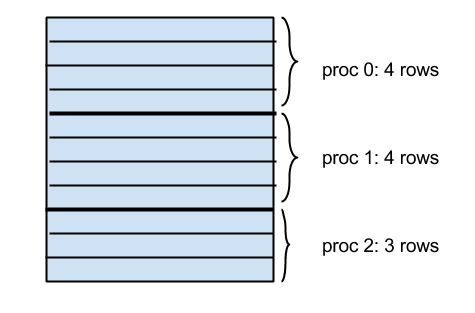
\includegraphics[scale=0.5]{finalPresentation/pics/rows-procs.png}}
	\end{picture}
\end{frame}

\begin{frame}{Kommunikation über "ghost rows"}
	\begin{picture}(0,0)
		\put(30,-80){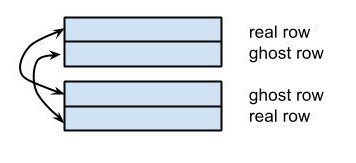
\includegraphics[scale=0.9]{finalPresentation/pics/real-ghost-rows.jpg}}
	\end{picture}
\end{frame}

\begin{frame}[fragile]{Parallelisierungsschema}
	\begin{picture}(0,230)
		\put(-120,0){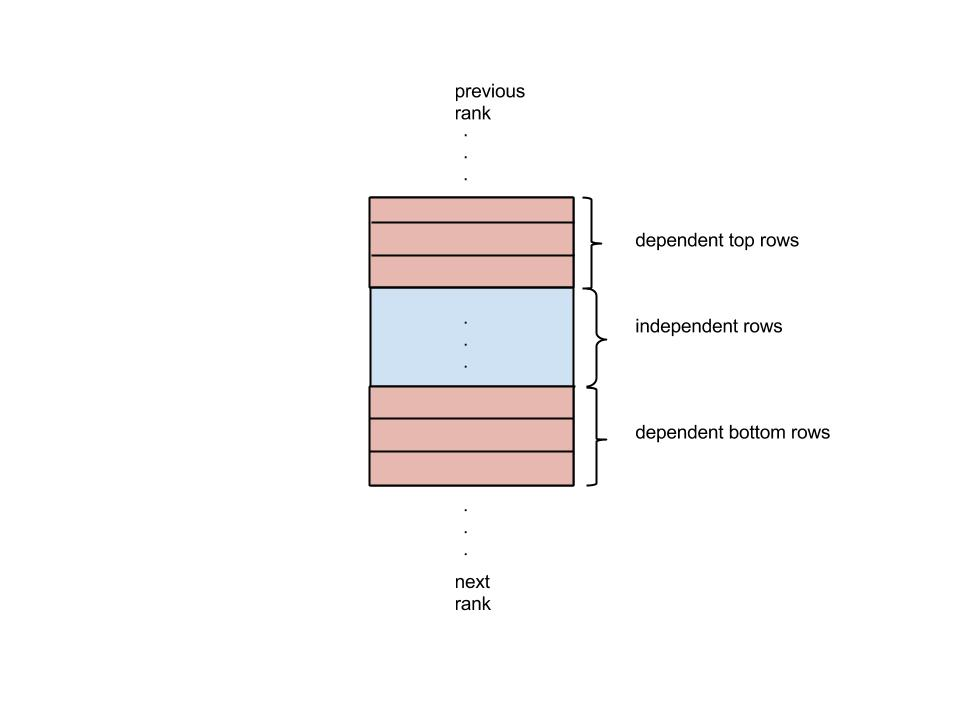
\includegraphics[height=8cm]{finalPresentation/pics/dependent-rows.jpg}}
		\put(170,180){\begin{minipage}[t]{0.4\linewidth}{
			\begin{itemize}
				\item[1.] Bewegung der independent ideas
				\item[2.] Bewegung der top dependent ideas, Kommunikation dieser
				\item[3.] Bewegung der bottom dependent ideas, Kommunikation dieser
			\end{itemize}
			}
		\end{minipage}}
	\end{picture}
\end{frame}

\begin{frame}[fragile]{Parallelisierungsschema}
\begin{lstlisting}[language=C,basicstyle=\small,keywordstyle=\color{black}]
#define send_ideas(ideas_arr, to, tag, req) 
  MPI_Isend(ideas_arr, num_cols, 
    mpi_idea_type, to, tag, MPI_COMM_WORLD, &req) 

#define receive_ideas_into(ideas_arr, from, tag, req) 
  MPI_Irecv(ideas_arr, num_cols, 
    mpi_idea_type, from, tag, MPI_COMM_WORLD, &req) 
\end{lstlisting}

\end{frame}

\begin{frame}[fragile]{Parallelisierungsschema}
\begin{lstlisting}[language=C,basicstyle=\small,breaklines=true,keywordstyle=\color{black}]
#define mpi_define_idea_type()                                               
  int blocklengths[5] = {1,1,1,1,1};                                  
  MPI_Datatype types[5] = {MPI_INT,MPI_INT,MPI_INT, MPI_INT, MPI_INT};       
  MPI_Datatype mpi_idea_type;                                                
  MPI_Aint offsets[5];                                                   
  offsets[0] = offsetof(Idea, a);                                            
  offsets[1] = offsetof(Idea, b);                                            
  offsets[2] = offsetof(Idea, c);                                            
  offsets[3] = offsetof(Idea, h);                                            
  offsets[4] = offsetof(Idea, empty);                                        
    MPI_Type_create_struct(5, blocklengths, offsets, types, &mpi_idea_type); 
    MPI_Type_commit(&mpi_idea_type);                                         
\end{lstlisting}
\end{frame}

\begin{frame}[fragile]{MPI-Code Überblick}
\begin{lstlisting}[language=C,basicstyle=\tiny,breaklines=true,keywordstyle=\color{black}]
  // INDEPENDENT ROWS
  if (num_rows >= 7) move_ideas(2, num_rows-5);
  barrier();

  // DEPENDENT ROWS TOP
  move_ideas(0, 3); 
  barrier();

  send_top_rows(field_new);
  receive_into_bottom_rows(field_new);
  barrier();

  // DEPENDENT ROWS BOTTOM
  move_ideas(num_rows - 4, 3);  
  barrier();

  send_bottom_rows(field_new);
  receive_into_top_rows(field_new);
  barrier();

  copy_field_new_into_field();
\end{lstlisting}
\end{frame}

\begin{frame}{Implementation Visualisierung}
	\begin{itemize}
		\item lokal mit Python/Pygame
		\item Output von C pro rank in out/\$round-\$rank files
		\item im Nachhinein: Rundenweise Einlesen der Files im Pygame-Loop
		\item Problem mit Integration des Clusters: rsync bottleneck
	\end{itemize}
\end{frame}

\begin{frame}{Optimierung}
	\begin{itemize}
		\item Ersetzen von Send/Recv mit Isend/Recv (10 \% Speedup)
		\item field / field\_new Kopieren per memcpy: fail
    \item Generell: gefühlte Fragilitaet von MPI Code bewog zu defensivem Verhalten - bloß nichts mehr kaputt machen (Beispiel: lieber mehr als zuwenig Barriers)
    \item Motivationsmangel: Performance von C eh mehr als ausreichend, Bottleneck bei
      Visualisierung und rsyncing vom Cluster
	\end{itemize}
\end{frame}

\section{Resultate und Messungen}
\begin{frame} {Profiling IO vs no IO absolut}
	\begin{picture}(0,0)
    \put(10,-100){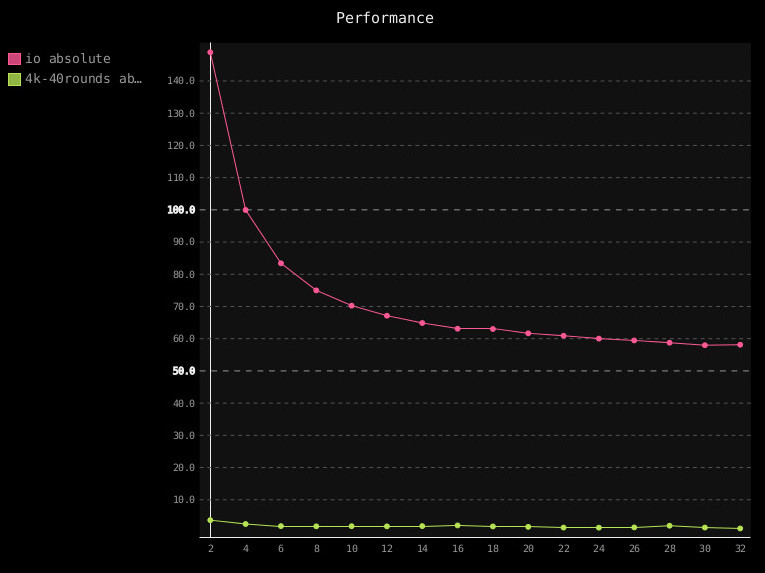
\includegraphics[scale=0.45]{finalPresentation/pics/io-vs-no-io-abs.jpg}}
	\end{picture}
\end{frame}

\begin{frame} {Performance IO vs no IO relativ}
	\begin{picture}(0,0)
    \put(10,-100){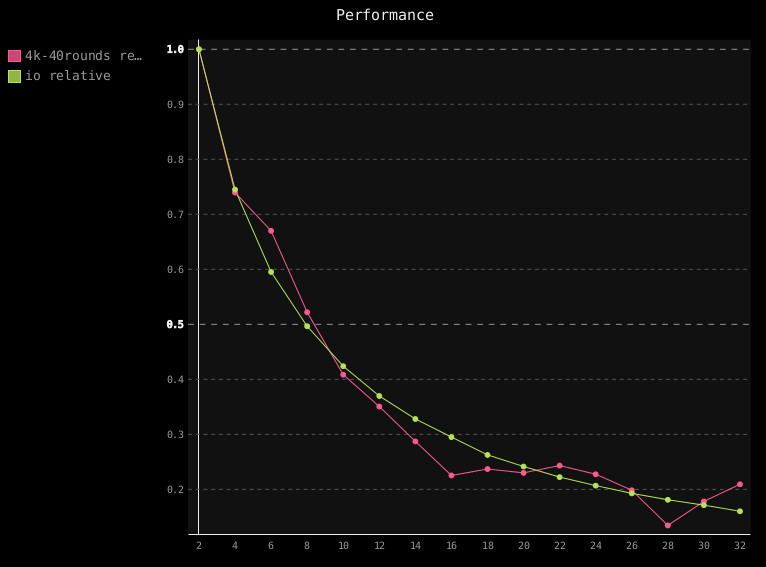
\includegraphics[scale=0.45]{finalPresentation/pics/io-vs-no-io-rel.jpg}}
	\end{picture}
\end{frame}

\begin{frame} {Performance IO vs no IO relativ}
	\begin{picture}(0,0)
    \put(10,-100){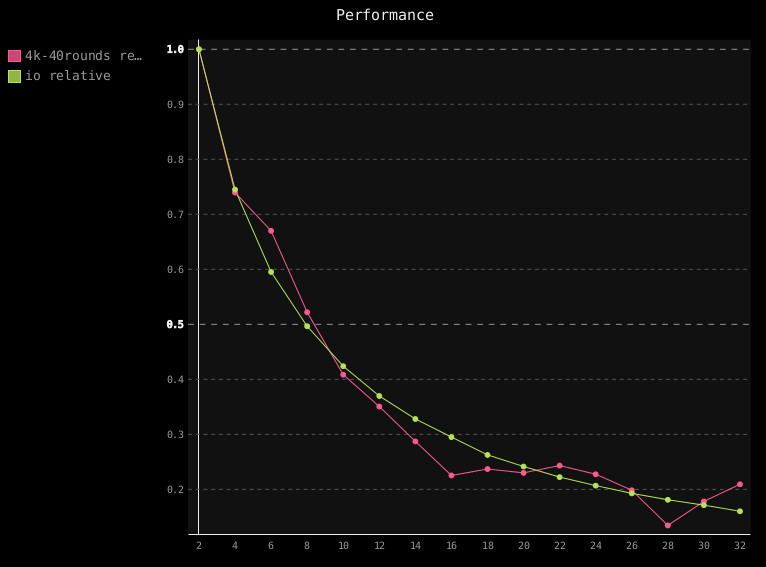
\includegraphics[scale=0.45]{finalPresentation/pics/io-vs-no-io-rel.jpg}}
	\end{picture}
\end{frame}

\begin{frame} {Performance no IO absolut}
	\begin{picture}(0,0)
    \put(10,-100){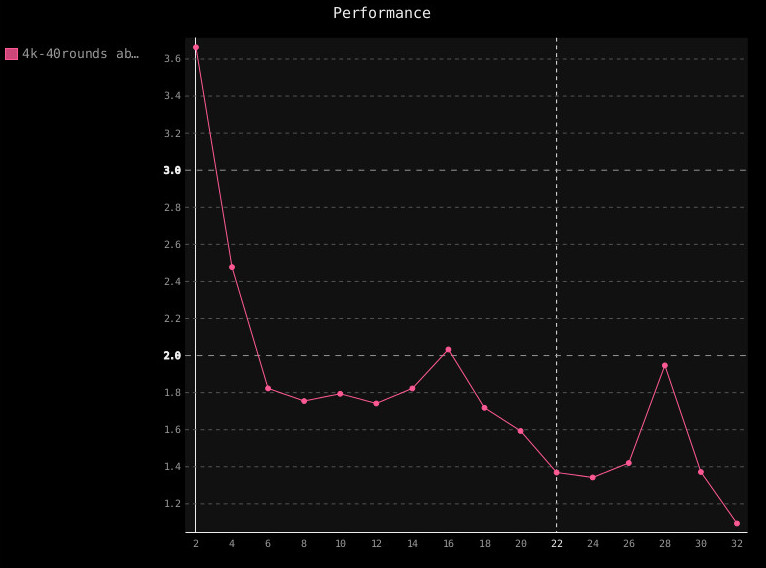
\includegraphics[scale=0.45]{finalPresentation/pics/perf-abs.jpg}}
	\end{picture}
\end{frame}


\section{Demo}
\begin{frame} {Ideen WV Farbcodierung}
	\begin{picture}(0,0)
    \put(10,-100){
\includegraphics[scale=0.45]{finalPresentation/pics/colors.jpg}}
	\end{picture}
\end{frame}
\begin{frame} {Demo}
\end{frame}


\begin{frame} {Inhaltliche Erkenntnisse}
	\begin{itemize}
		\item Qualität nimmt über die Zeit zu
		\item Obwohl andere selten vollständig entfernt, bilden 2-3 Ideen eine Majorität aus
		\item Qualität/Elaborationsgrad nimmt über die Zeit zu
		\item Es bleiben einige Menschen mit Ideen niedriger Qualität
		\item Selten: Durch Mutation entwickelt sich eine verdrängte Idee zur dominanten
	\end{itemize}
\end{frame}

\section{Probleme}

\begin{frame}{Probleme}
	\begin{block}{Probleme beim Debuggen}
		\begin{itemize}
			\item Logik und Bewegung größtenteils unter Beteiligung von Zufallselementen
			\item oft nicht reproduzierbare Bugs 
		\end{itemize}
	\end{block}
	
	\begin{block} {Real-Time Visualisierung}
		\begin{itemize}
			\item große Datenmenge
			\item Uns war nicht klar wie/ob X-Forwarding mit dem Cluster funktioniert wird
		\end{itemize}
	\end{block}
\end{frame}

\section{Fazit}

	

\end{document}
